\chapter{Image Reconstruction}\label{Image Reconstruction}\noindent

In the previous chapter we have developed tools that allow us to predict
and calculate the X-ray diffraction pattern from an arbitrary electron density,
using mild assumptions, namely that we are sufficiently far from the scatterer
that the Fraunhofer approximation holds and that there is no multiple
scattering.
In this chapter we will try to tackle the {\em inverse
  problem}, that is, from an arbitrary diffraction pattern we will try to
recover the electron density that gave rise to it.
\section{The Phase Problem}

We have seen that a diffraction pattern can be calculated from the Fourier
transform of the electron density. We have also seen in chapter
\ref{fourier_transform_basics} that the inverse of the Fourier transform is
exactly like the Fourier transform, except with the sign of the exponent
swapped. So we should be able to recover the electron density by,
\begin{equation}
\rho(\mathbf r) = \int_{\mathbf r} F(\mathbf S) \exp\left(-2
    \pi i \mathbf r \cdot \mathbf S \right) d\mathbf S\, .
\end{equation}

In general $F(\mathbf S)$ is a complex number and unfortunately it is not
possible to measure $F(\mathbf S)$, but only its absolute value, also known as
amplitude. The phase, also known as the argument of $F(\mathbf S)$, is not known and so
this problem is often called the {\em phase problem}. One could try to reconstruct the
object assuming that the phases have an arbitrary value, say 0, and use the
experimental amplitudes, the square root of the measured intensities, but this usually gives an uninterpretable picture. On
the other hand if the phases were known and the amplitudes unknown, then the
resulting picture is still quite similar to the original, suggesting that the
phases carry more structural information than the amplitudes (see Fig. \ref{Fig:PhaseSwapping}).
\begin{figure}[h]
  \centering
  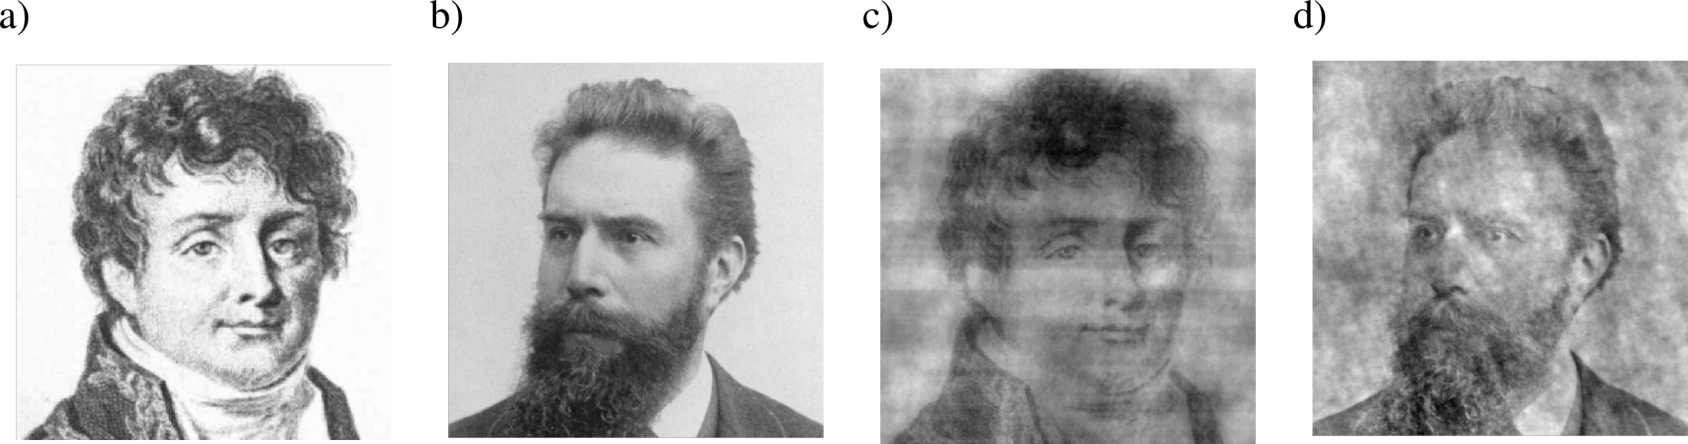
\includegraphics[width=1 \columnwidth]{Image_Reconstruction/PhaseSwapping2.png}
  \caption{Portraits of Jean-Baptiste Fourier (a) and Wilhelm R\"{o}ntgen (b).
    {\bf c)} Fourier synthesis using the amplitudes from b and the phases from
    a. {\bf d)}
    Fourier synthesis using the amplitudes from a and the phases from b.}
  \label{Fig:PhaseSwapping}
\end{figure}

If nothing about the object being imaged is known then the problem is
undetermined. For for a pattern with $N$ pixels we have $2N$ unknowns (the real and
imaginary part of the object) but only $N$ constraints. But if we know that the object is isolated, meaning the
object is surrounded by a constant $\rho$ (e.g., sample in vacuum with a
surrounding $\rho = 0$), then in some circumstances it is possible to solve this
problem. The number of pixels of the object must at least be half of that of the
diffraction pattern for the number of unknowns to match the number of
constraints, that is the oversampling ratio (see
Fig. \ref{Fig:OversamplingRatio}) of the image must be equal to or bigger than
two, or equivalently the object must occupy less than half of the field of
view. We will call images which fulfill this condition {\em oversampled}.

But this is not enough being able to solve the problem. In fact it
has long been known that the problem is often undetermined in the one dimension case
\cite{Walther1963Question}. Fortunately for higher dimensions it has
been proven that most oversampled patterns have unique solutions
\cite{Bruck1979Ambiguity}. This difference derives from the fact that one-dimensional
polynomials are factorizable unlike two or higher dimension ones.

\section{Image Reconstruction Algorithms}

Knowing that the two or higher dimensional phasing problem for oversampled
patterns has a unique solution in most cases can serve as a starting point to
solve the phase problem, but a method to find that unique solution is still
necessary. The phase problem is remarkably difficult since it is neither a
linear nor a convex problem. That makes it a nonconvex problem in a very high
dimensional space, which is a class of problems that is very challenging.

\begin{figure}[h]
  \centering
  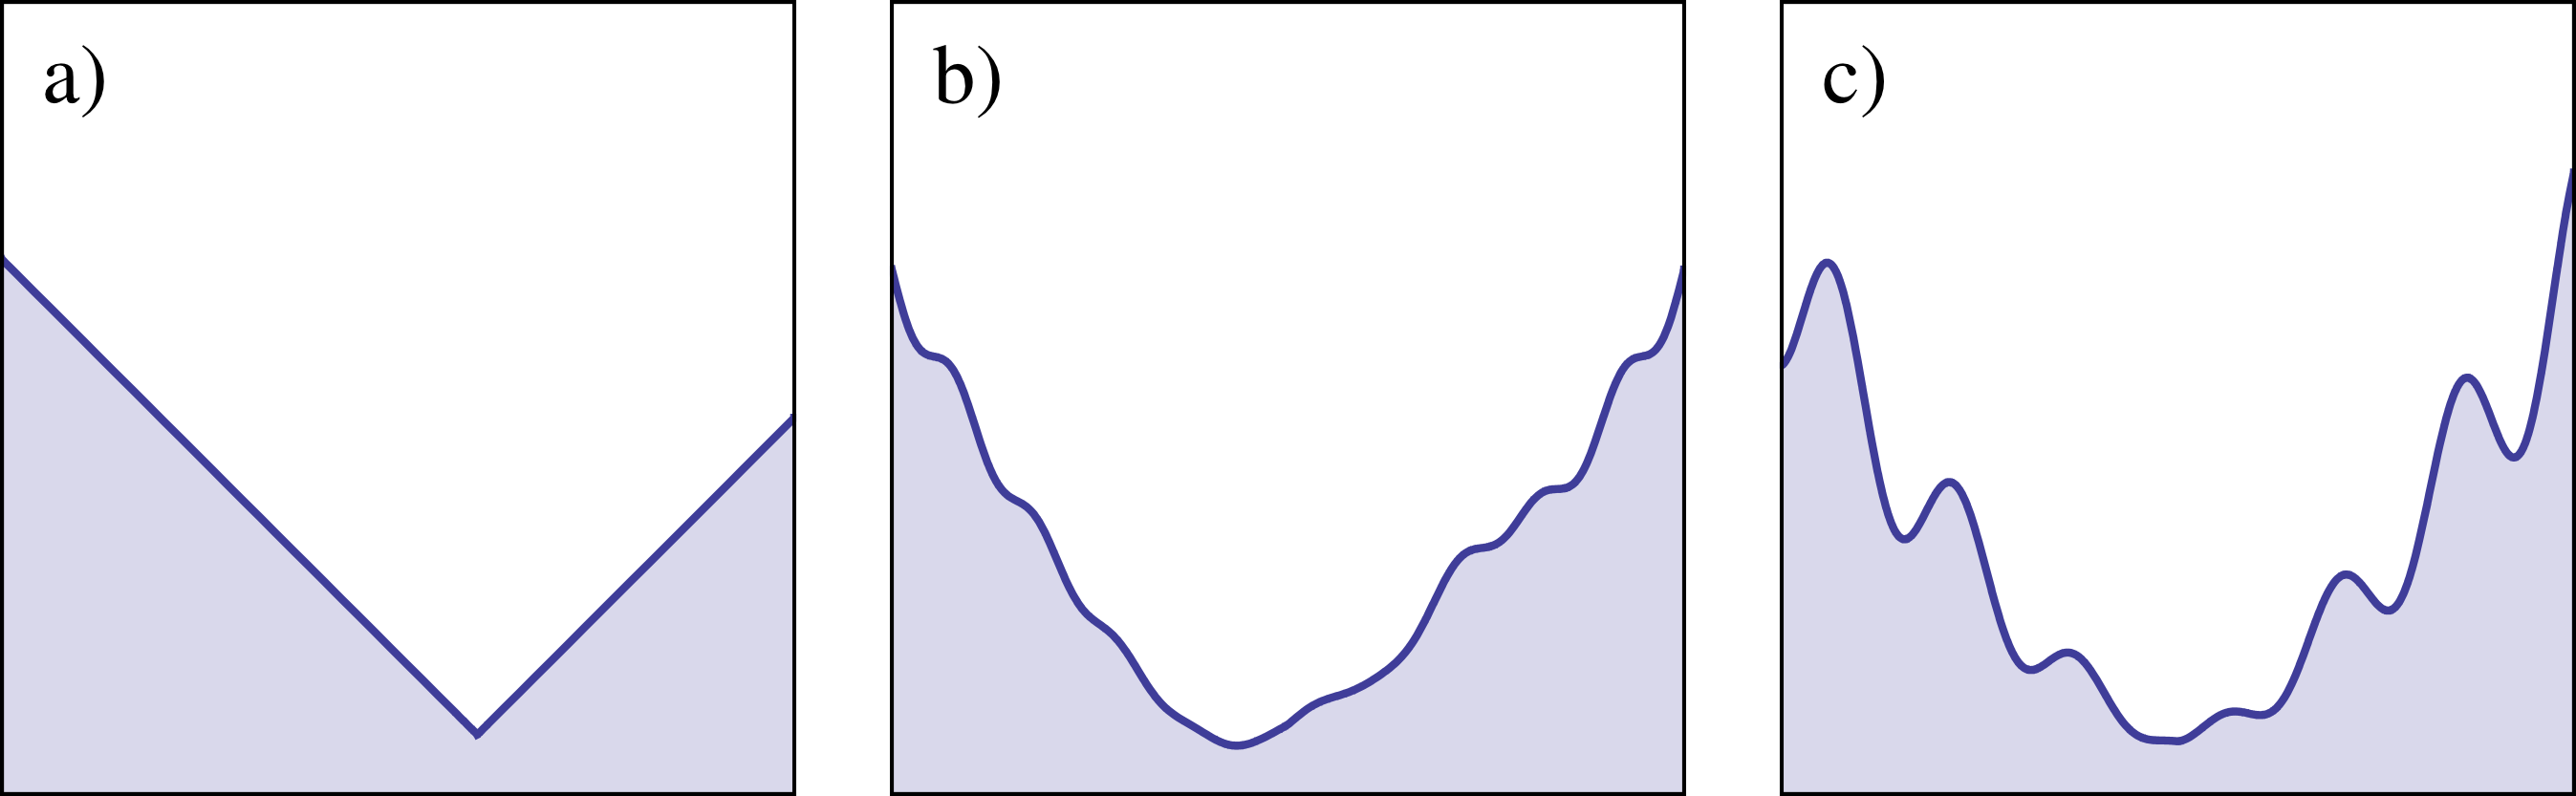
\includegraphics[width=1 \columnwidth]{Image_Reconstruction/convexity.png}
  \caption{Function to be minimized for a linear (a), convex (b) and nonconvex
    (c) optimization problems.}
  \label{Fig:Convexity}
\end{figure}

In 1972 Gerchberg and Saxton \cite{Gerchberg1972Practical} introduced an iterative algorithm to solve
a related problem, that of obtaining phase information using both the
diffraction pattern and an electron micrograph of a sample. The iteration starts
by Fourier transforming the real space input, $\rho_i(\mathbf x)$. Then it
replaces the resulting amplitudes with the square root of the intensities,
$I(\mathbf S)$. The result is then back Fourier transformed and the amplitudes
of the resulting images are replaced by the ones from the electron micrograph $M(\mathbf r)$.
\begin{algorithm}
\caption{Gerchberg-Saxton Iteration}
\begin{algorithmic}
  \STATE $F_{i}(\mathbf S) \gets \mathscr{F}\{\rho_i(\mathbf r)\}$
  \STATE $F_{i+1}(\mathbf S) \gets \sqrt{I(\mathbf S)} \frac{F_i(\mathbf S)}{|F_i(\mathbf S)|}$
  \STATE $\rho_{i+1}(\mathbf r) \gets M(\mathbf r)
  \frac{\mathscr{F}^{-1}\{F_{i+1}(\mathbf
    S)\}}{|\mathscr{F}^{-1}\{F_{i+1}(\mathbf S)\}|}$
\end{algorithmic}
\end{algorithm}

In 1978 Fienup \cite{Fienup1978Reconstruction}, inspired by the above algorithm, introduced on error
reduction algorithm to solve the phasing problem. Instead of using the electron
micrograph as constraints in real space Fienup introduces the concept of a {\em
  support} function, $\Pi(\mathbf r)$, which is equal to 1 where the
object is allowed to reside and 0 otherwise. 
The iteration is analogous to the Gerchberg-Saxton Iteration but the last step is replaced
by setting all points outside the support to 0.
\begin{algorithm}
\caption{Error Reduction Iteration}
\begin{algorithmic}
  \STATE $F_{i}(\mathbf S) \gets \mathscr{F}\{\rho_i(\mathbf r)\}$
  \STATE $F_{i+1}(\mathbf S) \gets \sqrt{I(\mathbf S)} \frac{F_i(\mathbf S)}{|F_i(\mathbf S)|}$
  \STATE $\rho_{i+1}(\mathbf r) \gets \Pi(\mathbf r) \mathscr{F}^{-1}\{F_{i+1}(\mathbf S)\}$
%  \STATE $i = 0$
\end{algorithmic}
\end{algorithm}

By applying this procedure iteratively it is possible to recover the correct
solution. 
Unfortunately
often 
 in practise the algorithm easily gets stuck in
local minima and cannot find the global minimum.

\subsection{Iterations as Projections}

In 1984 Levi and Stark realized that the above iterations can be
interpreted as projections in Hilbert space \cite{Levi1984Image}. This provides a
particularly powerful method for trying to understand these algorithms.
Let's call the replacement of the Fourier space amplitudes with the square root of
the intensities the modulus projection, $P_m$, and the replacement of the image
outside of the support with 0 the support projection, $P_s$. If one treats the
real space image as a vector in a high dimensional space, with one dimension per
pixel, then it is easy to see that $P_s$ is the projection into the hyperplane
spanned by the dimensions corresponding to pixels inside the support. The
modulus projection can also be interpreted as a projection in the space of the
pixels of the diffraction pattern, where each pixel contributes two dimensions,
the real part and the imaginary part (see Fig. \ref{Fig:Projections}). 

\begin{figure}[h]
  \centering
  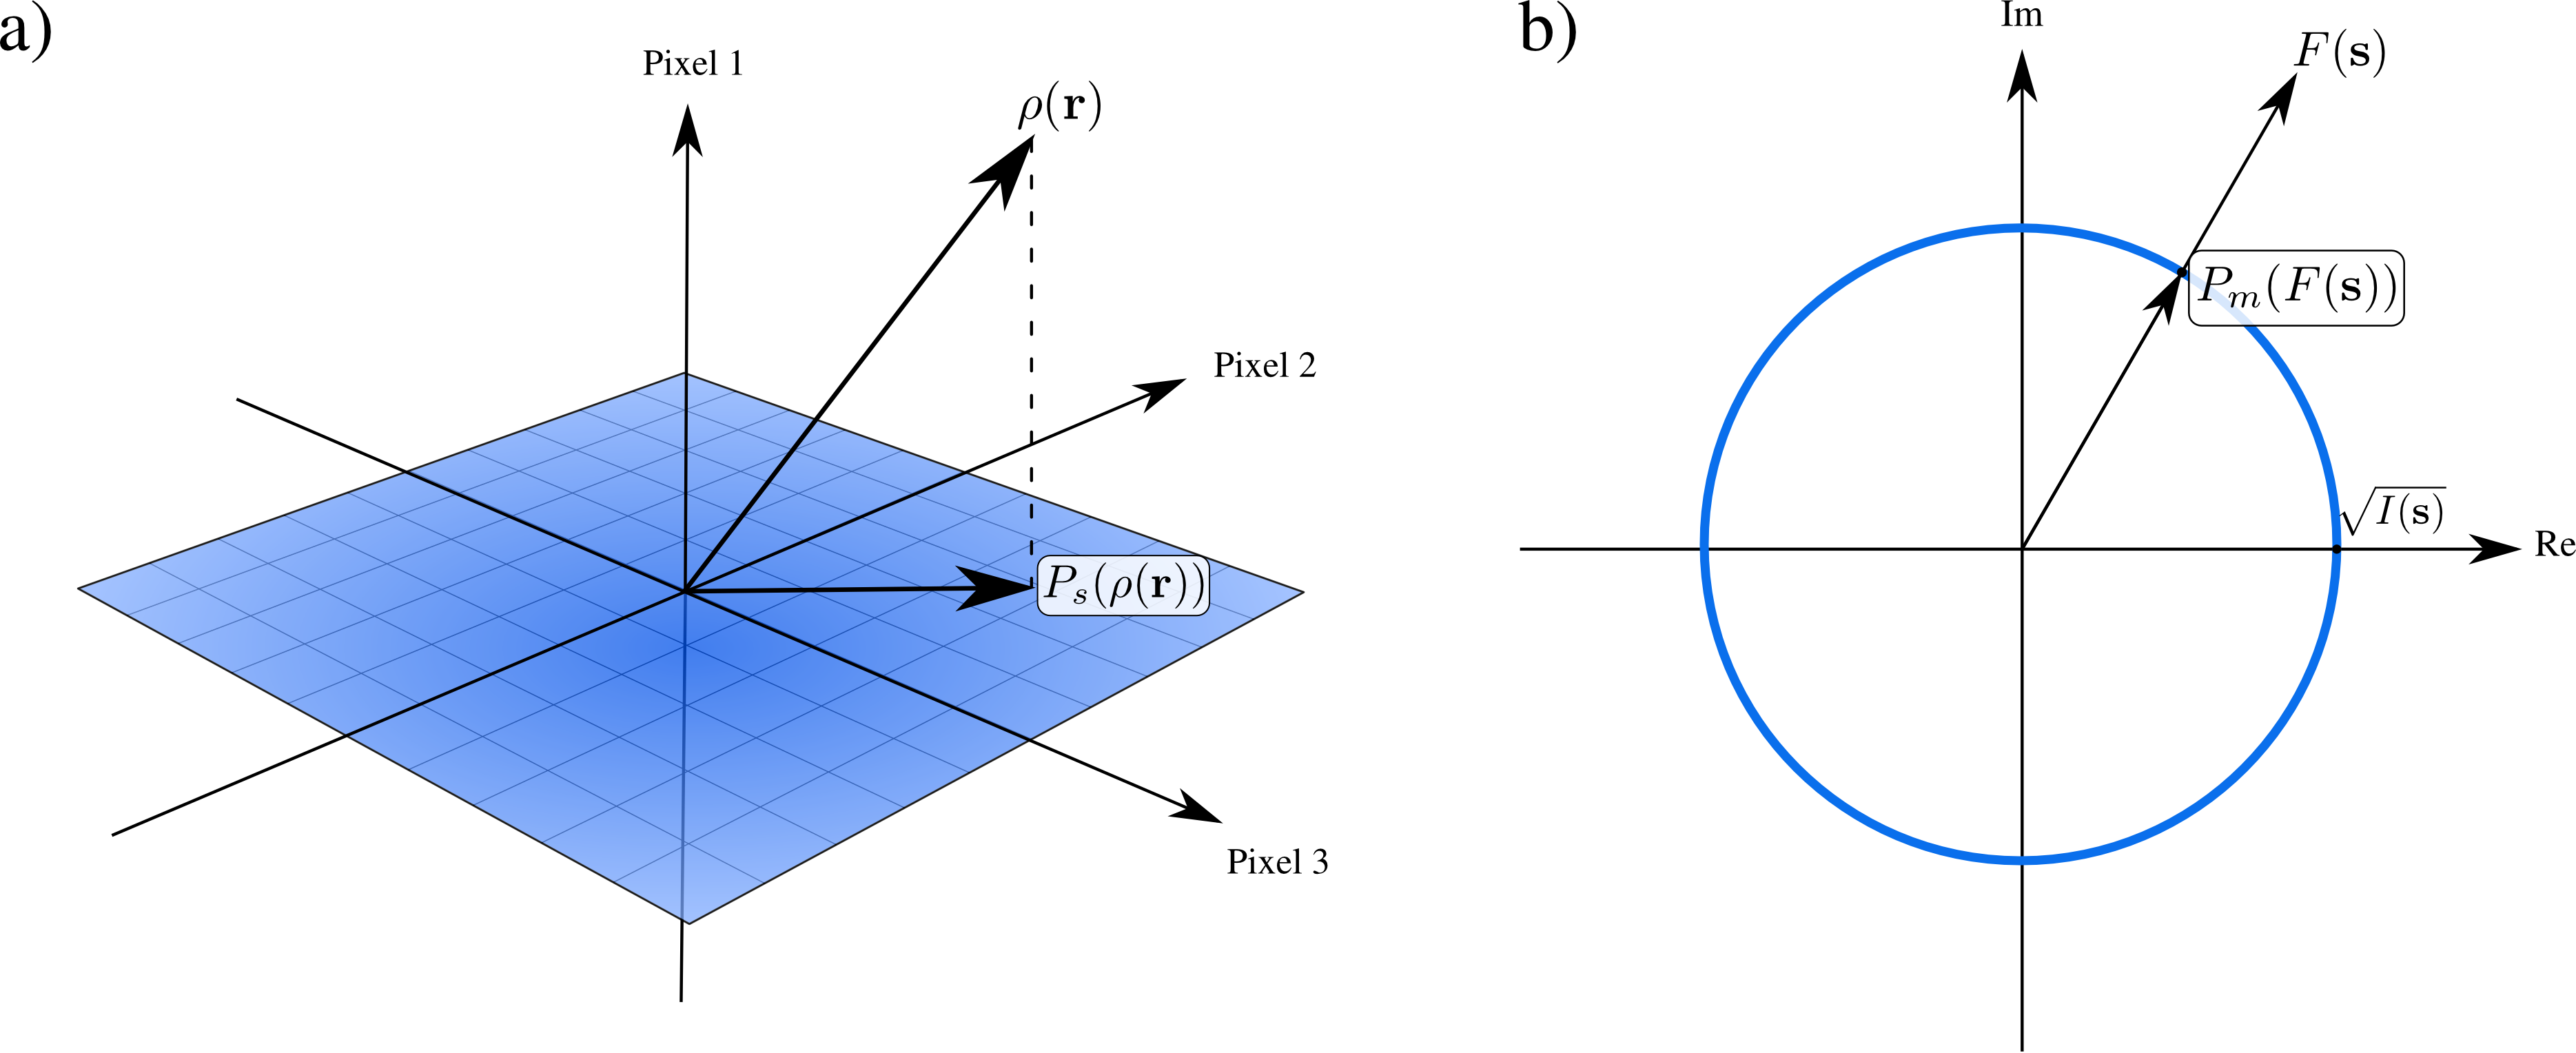
\includegraphics[width=1 \columnwidth]{Image_Reconstruction/projections.png}
  \caption{{\bf a)} Support projection for a 3 pixel image where the support is
    composed of pixels 2 and 3. {\bf b)} Modulus projection for 1 pixel of the
    diffraction pattern.}
  \label{Fig:Projections}
\end{figure}

Due to the distance preserving property of the Fourier transform the modulus
projection is also a projection in real space. The biggest difference between
the two projection is that while the support constraint set is convex, the
modulus constraint is not, that is to say, not all points between two points of the modulus
constraint set belong to the modulus constraint set.

In this framework of projections the Error Reduction algorithm is simply the
modulus projection ($P_m$) followed by the support projection ($P_s$). The fact that it stagnates can then be easily understood in
connection to the non convexity of the modulus constraint as
Fig. \ref{Fig:Stagnation} illustrates.

\begin{figure}[h]
\centering
  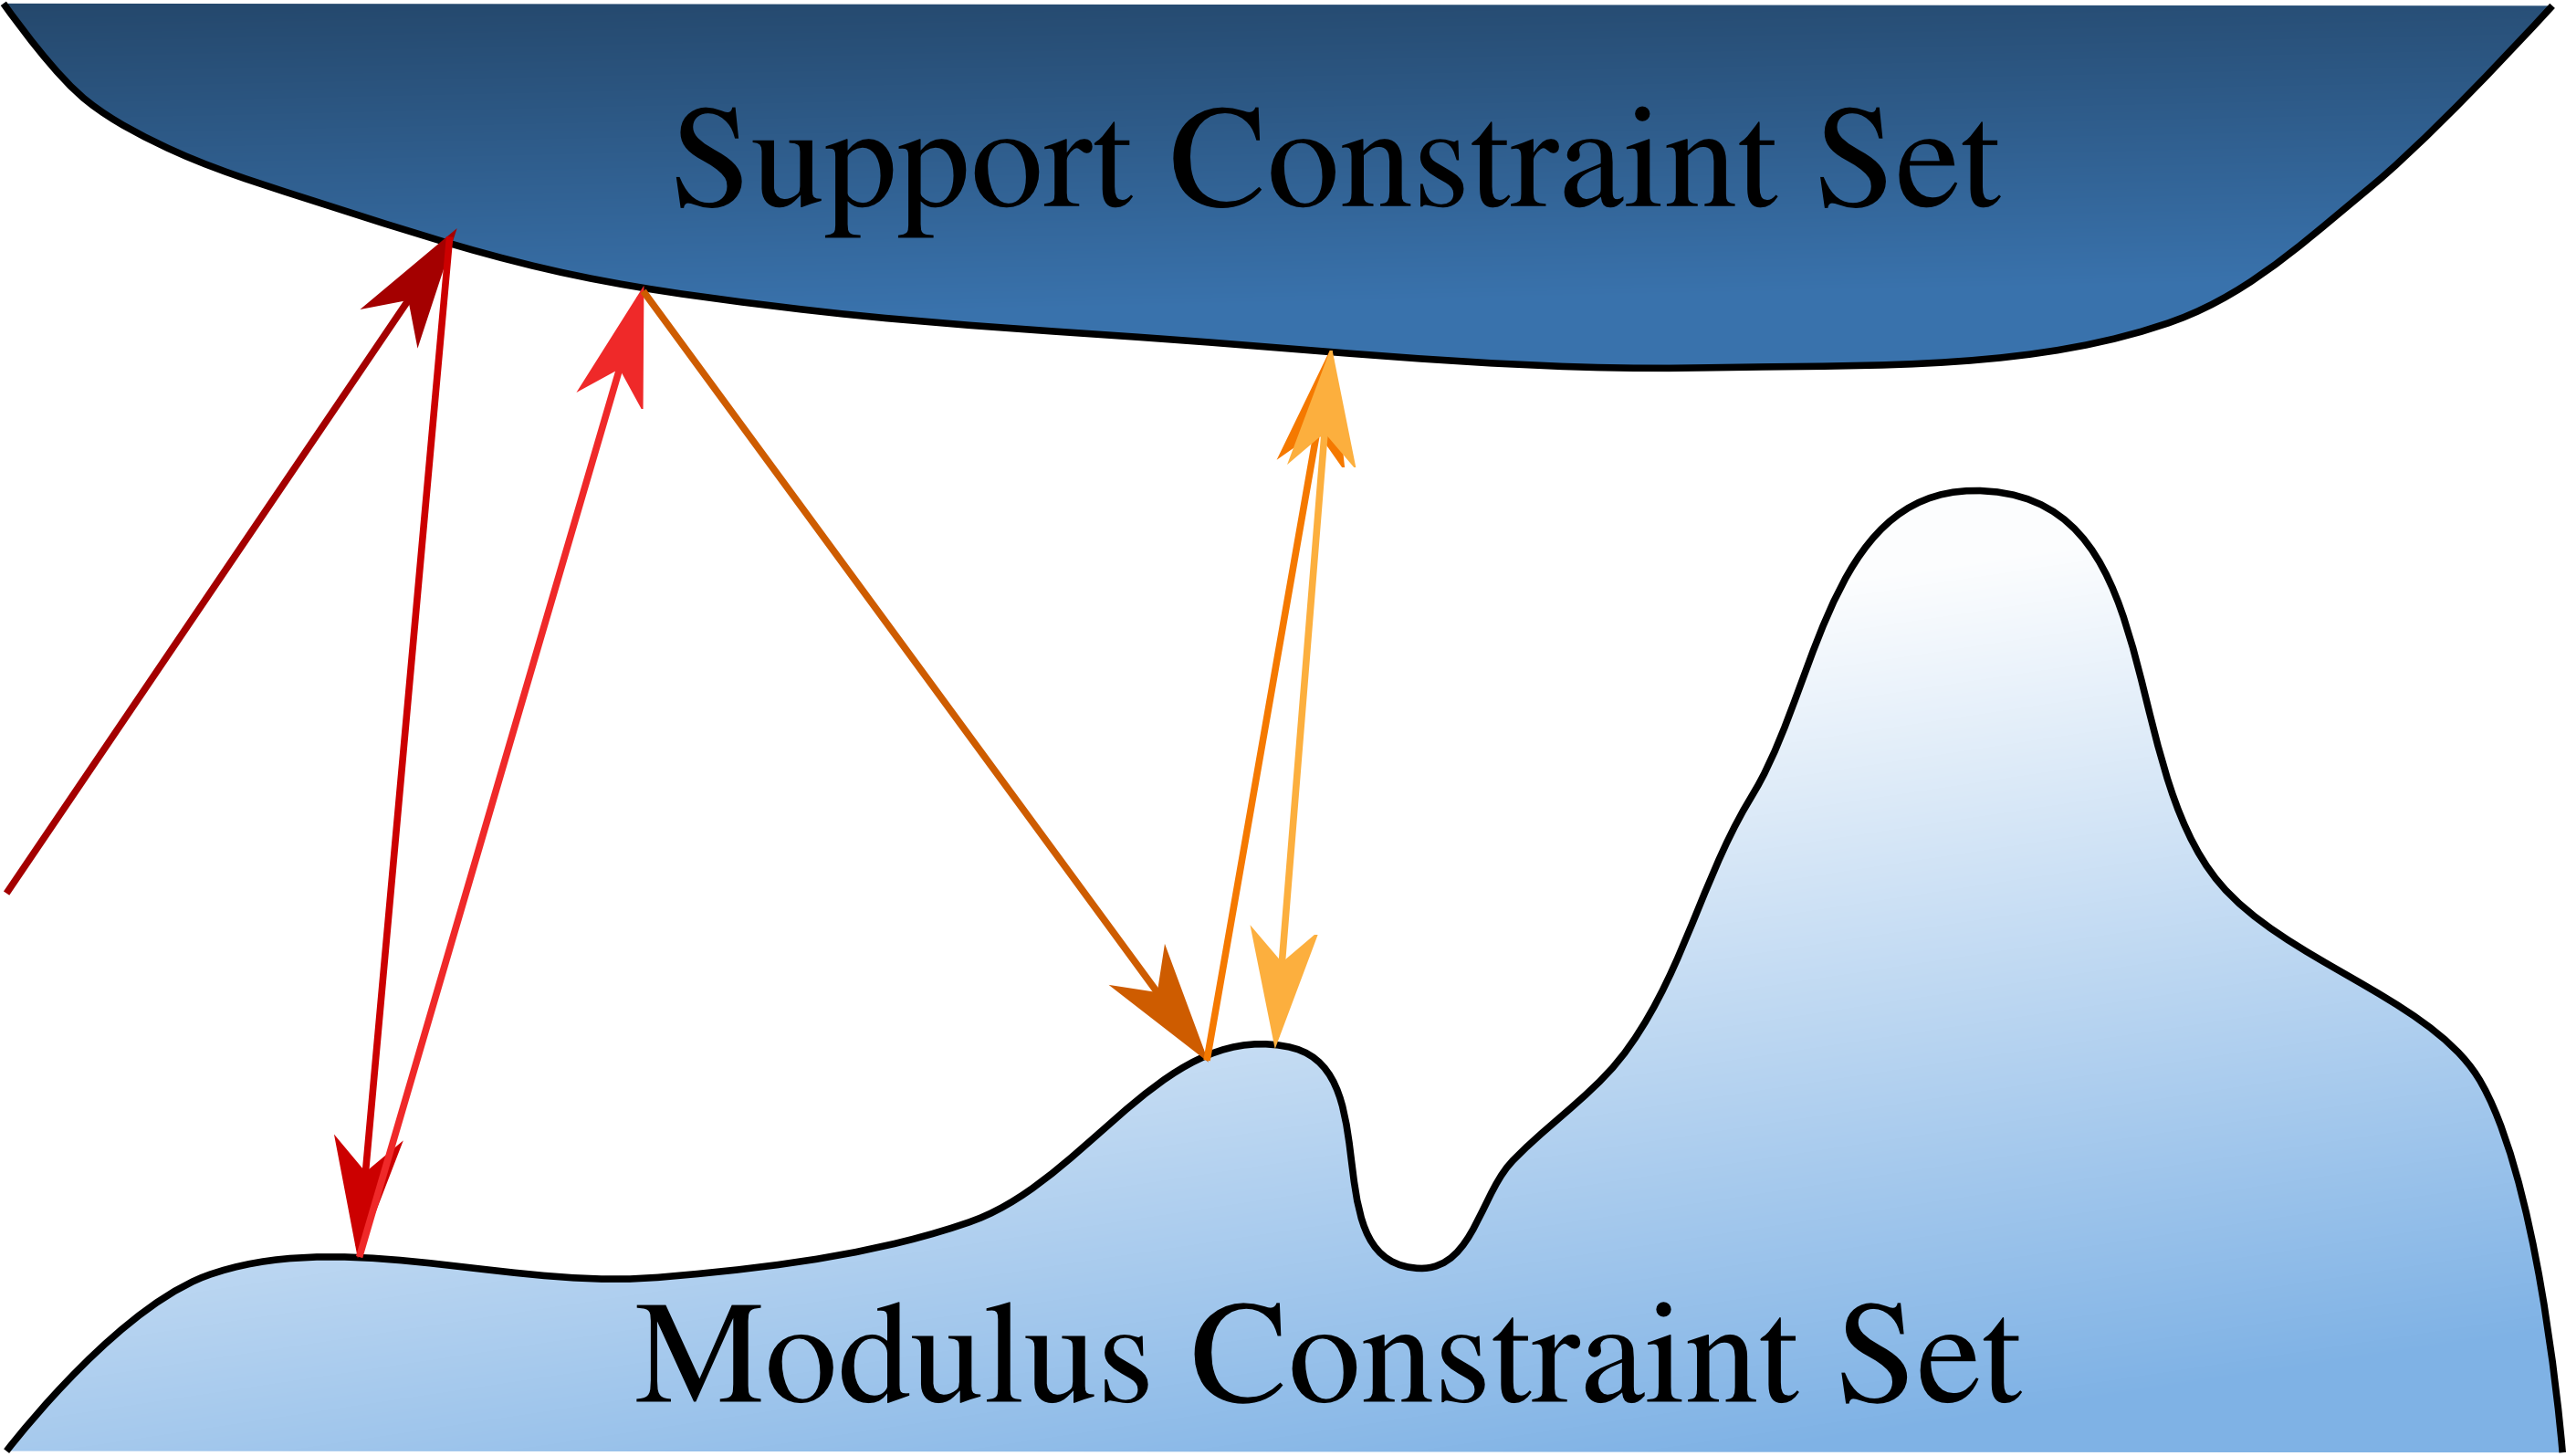
\includegraphics[width=0.8 \columnwidth]{Image_Reconstruction/Stagnation.png}
  \caption{Successive iterations of the Error Reduction algorithm represented as
    vectors of different color. The algorithm stagnates on a local minimum due
    to the non convexity of the modulus constraint set.}
  \label{Fig:Stagnation}
\end{figure}

In 1982 Fienup introduced the Hybrid Input-Output(HIO) algorithm \cite{Fienup1982Phase}
which is defined as:
\begin{algorithm}
\caption{Hybrid Input-Output Iteration}
\begin{algorithmic}
  \STATE $F_{i}(\mathbf S) \gets \mathscr{F}\{\rho_i(\mathbf r)\}$
  \STATE $F_{i+1}(\mathbf S) \gets \sqrt{I(\mathbf S)} \frac{F_i(\mathbf
    S)}{|F_i(\mathbf S)|}$
  \STATE $\rho^{\prime}(\mathbf r) \gets \mathscr{F}^{-1}\{F_{i+1}(\mathbf S)\}$
  \STATE $\rho_{i+1}(\mathbf r) \gets \Pi(\mathbf r) \rho^{\prime}(\mathbf r) +
  (1-\Pi(\mathbf r)) (\rho_i(\mathbf r)-\beta \rho^{\prime}(\mathbf r))$
%  \STATE $\rho_{i+1}(\mathbf r) \gets \rho^{\prime}(\mathbf r) - \left(1-\Pi(\mathbf r)\right) \beta \rho^{\prime}(\mathbf r)$
\end{algorithmic}
\end{algorithm}

which can also be represented with projection operators as \cite{Thibault2007Algorithmic}:
\begin{equation}
  \rho_{i+1} = \rho_{i} + \beta\left[P_s((1+\beta^{-1})P_m(\rho_i)-\beta^{-1}
    \rho_{i}) -P_m(\rho_i)\right] .
\end{equation}

This means that the change in each iteration is a sum of a point projected onto the
support constraint minus a point projected onto the modulus constraint all
scaled by a relaxation factor $\beta$ (see Fig. \ref{Fig:HIO_Iteration}). If the
separation between the two 
projections is large the step length will be large and the algorithm will
probably explore some other areas. This means that the algorithm is quite good
at getting out of local minima, but also means that if the sets never get too
close (due to noisy data for example), this algorithm will have a difficult time
keeping close to the best solution, even though it might pass through it.

\begin{figure}[h]
\centering
  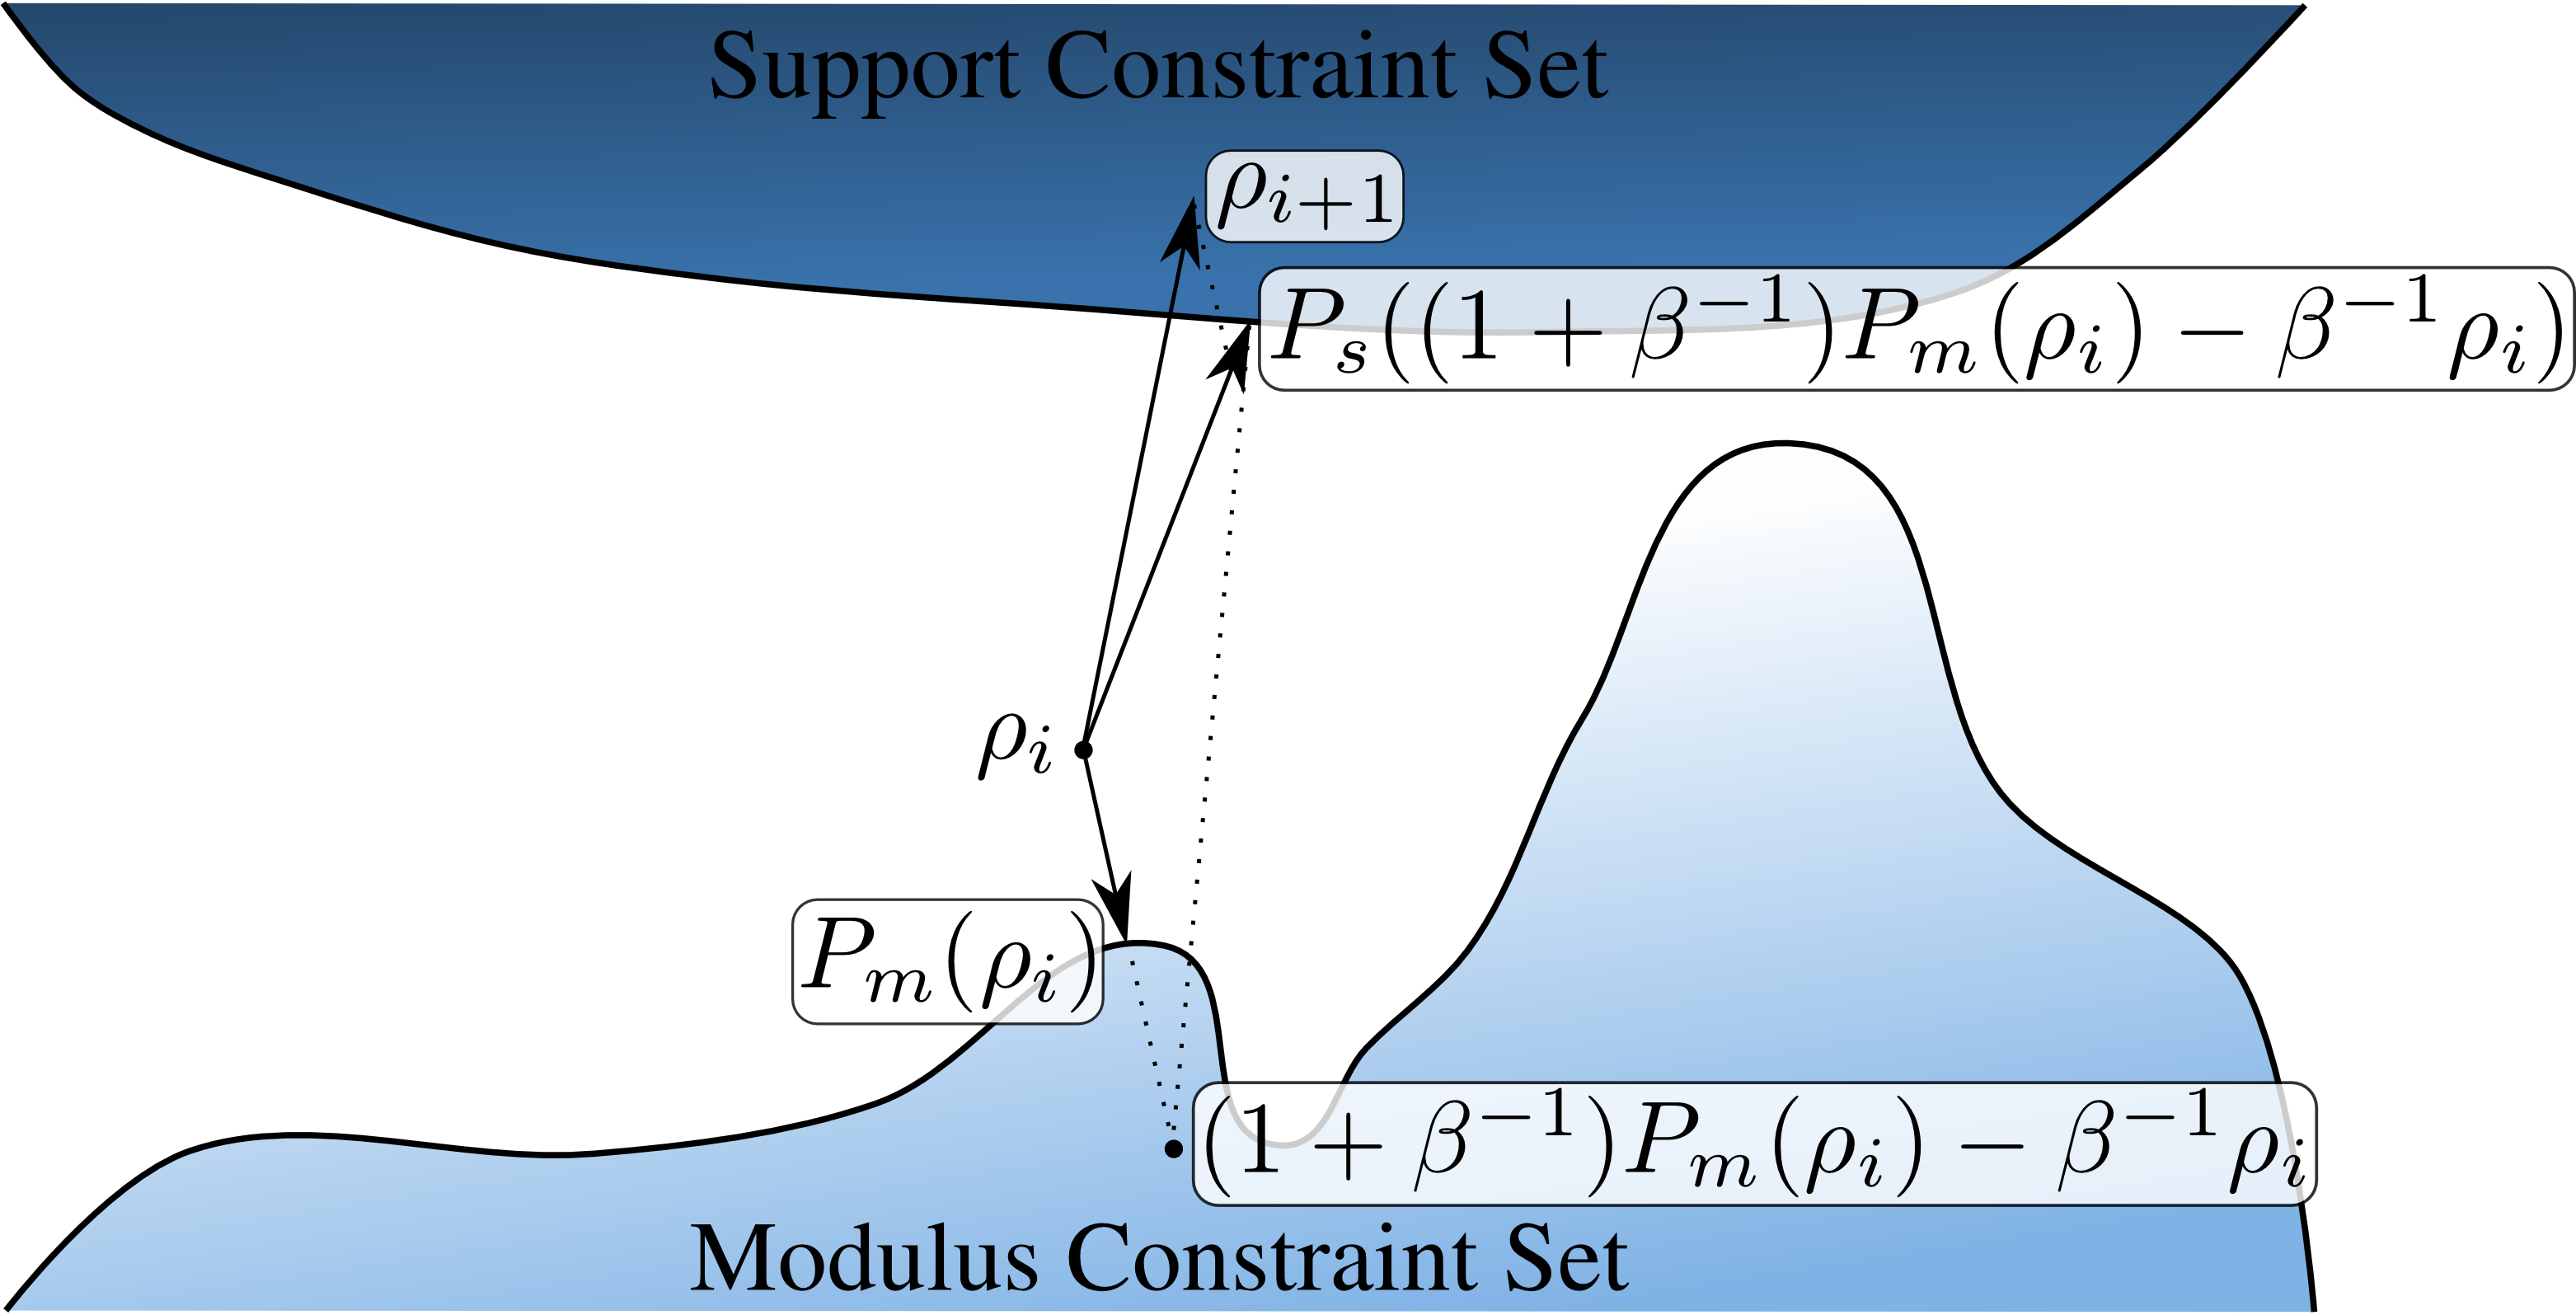
\includegraphics[width=0.9 \columnwidth]{Image_Reconstruction/hio_iteration.png}
  \caption{One iteration of the HIO algorithm assuming the origin is at
    $\rho_i$. Note that the iteration does not end at the surface of the
    constraint set.}
  \label{Fig:HIO_Iteration}
\end{figure}

The HIO algorithm was a tremendous improvement and it is still widely used
today. It is probably the most popular algorithm for phase retrieval. 

\subsection{Shrinkwrap algorithm}

While the HIO algorithm produces very good results when a tight support is known
for many applications it is hard to know in advance the shape of the support,
and a support that is too large can make phasing impossible in practice. 

In 2003 Marchesini \cite{Marchesini2003Xray} introduced the {\em Shrinkwrap
  algorithm} which does not require the support function as input and instead
tries to deduce it during the reconstruction. It does so by starting with a
support derived from the autocorrelation, where all pixels above a certain
threshold are included in the support. It then refines the support every $n$
iterations by blurring the current best guess of the object and keeping in the
support only those pixels that are above a certain threshold of the maximum pixel
value. The value of $n$ is typically a couple dozen iterations. The idea of the
algorithm is that even with a bad support some features of the objects will
start to show up, so it makes use of those recovered features to improve the
support. This algorithm has been remarkably successful in reconstructing several
experimental data sets
\cite{Chapman2006Highresolution,Barty2008Ultrafast,Barty2008Threedimensional}.

This algorithm was also used for image reconstruction in {\bf papers
\ref{cowboys},\ref{music} and \ref{dynamics}}.

\section{Image reconstruction software}

Even though there is a large number of algorithms and techniques published for
image reconstruction from CXDI diffraction patterns there is, to our knowledge, no publicly available
software package that integrates all these tools in an easy to use package.

Hawk, open source software package for data processing, being developed in Uppsala, is trying to fill
this gap ({\bf paper \ref{hawk}}). It is publicly available under the GNU General Public License at
\url{http://xray.bmc.uu.se/hawk}  and implements the following phasing algorithms:
 HIO \cite{Fienup1982Phase}, RAAR \cite{Luke2005Relaxed}, difference map
 \cite{Elser2003Phase}, HPR \cite{Bauschke2003Hybrid}, HAAR \cite{Bauschke2006Strongly}, ESPRESSO
\cite{Marchesini2008Ab} and charge flipping
\cite{Oszlanyi2004Ab,Oszlanyi2005It}. It is also
capable to leverage graphic processing units using CUDA providing very large speedups over classic
CPU based programs.

%%% Local Variables: 
%%% mode: latex
%%% TeX-master: "../Thesis"
%%% End: 
